% ============================================================
% arXiv version of the TER manuscript
% Same content as main.tex; article class, no cover page, no TOC.
% ============================================================
\documentclass[11pt,a4paper]{article}

% ---- Language and encoding ----
\usepackage[english]{babel}
\usepackage[utf8]{inputenc}
\usepackage[T1]{fontenc}

% ---- Fonts ----
\usepackage{mathpazo}
\usepackage[scaled]{helvet}
\usepackage{courier}

% ---- Colors ----
\usepackage{xcolor}
\definecolor{citegreen}{RGB}{0, 166, 79}
\definecolor{linkred}{RGB}{204, 51, 51}
\definecolor{urlcyan}{RGB}{0, 154, 180}

% ---- Math ----
\usepackage{amssymb}
\usepackage{amsmath}
\usepackage{braket}

% ---- Tables ----
\usepackage{tabularx}
\usepackage{booktabs}

% ---- Figures ----
\usepackage{graphicx}
\setkeys{Gin}{keepaspectratio}
\usepackage{float}
\usepackage{caption}
\usepackage{subcaption}

% ---- Lists ----
\usepackage{enumitem}

% ---- TikZ ----
\usepackage{tikz}
\usetikzlibrary{decorations.pathreplacing, arrows, positioning}
\usepackage{pgfplots}
\pgfplotsset{compat=1.18}

% ---- Layout: arXiv-standard 1-inch margins ----
\usepackage[margin=1in]{geometry}
\parskip=1.5mm
\parindent=0mm

% ---- Bibliography ----
\usepackage[numbers,sort&compress]{natbib}

% ---- Hyperlinks: arXiv-style boxes ----
\usepackage{hyperref}
\urlstyle{sf}
\hypersetup{
    colorlinks=false,
    citebordercolor=citegreen,
    linkbordercolor=linkred,
    urlbordercolor=urlcyan,
    pdfborderstyle={/S/U/W 1},
    pdftitle={Quantum Machine Learning for Zero-Day IoT Intrusion Detection},
    pdfauthor={Ashkan Motamedifar},
}

% ============================================================
% Map thesis heading levels to article heading levels.
% \chapter → \section, \section → \subsection, \subsection → \subsubsection
% This lets us reuse chapters/*.tex without rewriting them.
% ============================================================
\let\OldSection\section
\let\OldSubsection\subsection
\let\OldSubsubsection\subsubsection

\newcommand{\chapter}[1]{\OldSection{#1}}
\renewcommand{\section}[1]{\OldSubsection{#1}}
\renewcommand{\subsection}[1]{\OldSubsubsection{#1}}

% Silence \blankpage from main.tex (thesis-only helper)
\newcommand{\blankpage}{}

\title{Quantum Machine Learning for Zero-Day IoT Intrusion Detection\\
\large A comparison of QCNN, data re-uploading, autoencoder, and classical baselines
on the ToN\_IoT dataset}

\author{Ashkan Motamedifar\thanks{\texttt{ashkanmotamedifar@gmail.com}}\\
Laboratoire ICube, UMR 7357 --- CNRS\\
Universit\'{e} de Strasbourg, France}

\date{\today}

\begin{document}
\maketitle

\begin{abstract}
We compare quantum machine learning classifiers with classical baselines
for IoT network intrusion detection on the ToN\_IoT dataset, focusing on
\emph{zero-day} attack detection where models are tested on an attack class
never seen during training. Two quantum architectures are implemented
in PennyLane: a Quantum Convolutional Neural Network (QCNN, Hur et al.\
2022) on 8~qubits, and single-qubit and 4-qubit data re-uploading circuits
(P\'erez-Salinas et al.\ 2020). Classical baselines include SVM, Random
Forest, two feed-forward networks, and an autoencoder anomaly detector.
On the standard 3-class task (normal / DoS / injection), classical methods
dominate: Random Forest reaches 99\% accuracy while quantum models plateau
at 68--75\%. The picture inverts under zero-day evaluation: every supervised
classical baseline collapses below 3\%, while the QCNN reaches 68.6\% $\pm$
6.8\% on 7 of 10 seeds (3 hit barren plateaus), and an unsupervised autoencoder
matches at 70.5\% $\pm$ 14.4\%. The QCNN achieves this with 56$\times$ less
training data and lower variance when convergent, but pays a 30\% training-failure
rate. All quantum and autoencoder numbers are averaged over 10 random seeds
to expose initialization sensitivity. Results suggest that hierarchical
quantum feature maps and classical reconstruction-based detectors are
complementary routes to out-of-distribution generalization; the quantum
route is not (yet) clearly preferable, but performs comparably in a
regime where labelled normal traffic is scarce.
\end{abstract}

% ============================================================
% Body: reuse the same chapter files
% ============================================================

\chapter{Introduction}
\label{chap:introduction}

Machine learning has become a key tool for solving complex classification and prediction tasks across many domains, including network security. Classical models such as neural networks and support vector machines perform well, but their computational cost grows as datasets become larger and more complex. This raises the question of whether alternative computing paradigms could offer practical advantages.

Quantum computing exploits the physical phenomena of superposition and entanglement to process information in fundamentally different ways from classical computers. In recent years, researchers have proposed \emph{parameterized quantum circuits}~\cite{benedetti2019parameterized} as trainable models for machine learning, where quantum gate parameters are optimized in the same way as weights in a neural network. Two architectures are particularly relevant to this work: \emph{data re-uploading}~\cite{perez2020data}, which encodes classical data multiple times into a quantum circuit to build a universal classifier, and \emph{Quantum Convolutional Neural Networks} (QCNN)~\cite{hur2022quantum}, which adapt the classical CNN structure to quantum circuits with logarithmic depth.

These quantum models are designed to operate on current \emph{Noisy Intermediate-Scale Quantum} (NISQ) devices~\cite{preskill2018quantum}, which are limited in both the number of qubits and the circuit depth that can be reliably executed.

In this work, I apply quantum machine learning to \textbf{network traffic classification} using the ToN\_IoT dataset~\cite{toniot2020dataset}, which contains one million IoT network flow records labeled as normal traffic, Denial-of-Service (DoS) attacks, or injection attacks. The dataset is heavily imbalanced. Because zero-day detection is closer to anomaly detection than to closed-set classification, I additionally include an autoencoder trained on normal traffic only as an unsupervised baseline. I address the following objectives:

\begin{enumerate}[nosep]
    \item Compare quantum classifiers with supervised and unsupervised classical baselines on the same network dataset.
    \item Evaluate data re-uploading and QCNN architectures in terms of accuracy, parameter efficiency, and initialization sensitivity.
    \item Test the ability of these models to detect \emph{zero-day attacks}---attack types absent from the training data.
\end{enumerate}

All quantum experiments are implemented using PennyLane~\cite{pennylane}. The remainder of this manuscript covers quantum foundations (Chapters~2--3), the dataset and implementation (Chapters~4--5), results and conclusion (Chapters~6--7).
\chapter{Quantum Computing Foundations}
\label{chap:quantum_foundations}

This chapter introduces the quantum computing concepts that underpin the machine learning models used in this work. I cover qubits, quantum gates, measurement, data encoding strategies, parameterized quantum circuits, and the constraints of current quantum hardware.

% ============================================================
\section{Qubits and Superposition}
\label{sec:qubits}

In classical computing, the fundamental unit of information is the bit, which takes a value of either 0 or~1. In quantum computing, the analogous unit is the \emph{qubit}~\cite{nielsen2010quantum}. A qubit is a two-level quantum system whose state is a vector in a two-dimensional complex Hilbert space. The two basis states are denoted $\ket{0}$ and $\ket{1}$, and a qubit can exist in a \emph{superposition} of both:
\begin{equation}
    \ket{\psi} = \alpha \ket{0} + \beta \ket{1}, \qquad |\alpha|^2 + |\beta|^2 = 1,
    \label{eq:superposition}
\end{equation}
where $\alpha, \beta \in \mathbb{C}$ are complex amplitudes. The values $|\alpha|^2$ and $|\beta|^2$ represent the probabilities of obtaining outcomes 0 and~1 upon measurement.

Since global phase is unobservable, any single-qubit state can be parameterized by two angles $\theta \in [0, \pi]$ and $\varphi \in [0, 2\pi)$:
\begin{equation}
    \ket{\psi} = \cos\frac{\theta}{2}\,\ket{0} + e^{i\varphi}\sin\frac{\theta}{2}\,\ket{1}.
    \label{eq:bloch}
\end{equation}

This defines a point on the \emph{Bloch sphere} (Figure~\ref{fig:bloch_sphere}), a unit sphere in $\mathbb{R}^3$ where $\ket{0}$ is the north pole, $\ket{1}$ the south pole, and every quantum gate corresponds to a rotation of this sphere.

\begin{figure}[ht]
    \centering
    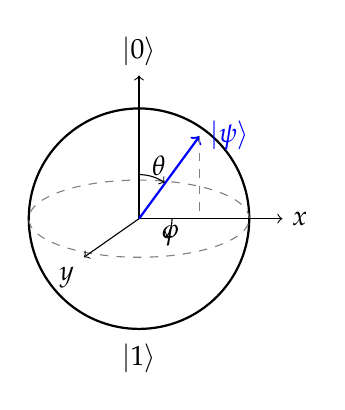
\begin{tikzpicture}[scale=1.4]
        \draw[thick] (0,0) circle (1);
        \draw[dashed, gray] (0,0) ellipse (1 and 0.35);
        \draw[->] (0,0) -- (1.3,0) node[right] {$x$};
        \draw[->] (0,0) -- (0,1.3) node[above] {$\ket{0}$};
        \draw[->] (0,0) -- (-0.5,-0.35) node[below left] {$y$};
        \node[below] at (0,-1.05) {$\ket{1}$};
        \draw[->, thick, blue] (0,0) -- (0.55, 0.75) node[right] {$\ket{\psi}$};
        \draw[dashed, gray] (0.55, 0.75) -- (0.55, 0);
        \draw[->] (0, 0.4) arc (90:54:0.4);
        \node at (0.18, 0.48) {$\theta$};
        \draw[->] (0.3, 0) arc (0:-35:0.3);
        \node at (0.28, -0.15) {$\varphi$};
    \end{tikzpicture}
    \caption{The Bloch sphere. Any pure single-qubit state $\ket{\psi}$ corresponds to a point on the surface, parameterized by angles $\theta$ and $\varphi$.}
    \label{fig:bloch_sphere}
\end{figure}
% ============================================================
\section{Multi-Qubit Systems and Entanglement}
\label{sec:multiqubit}
The joint state space of $n$~qubits is a $2^n$-dimensional Hilbert space. A general pure state can be written as
\[
\ket{\Psi} = \sum_{j=0}^{2^n-1} c_j \ket{j},
\qquad
\sum_{j=0}^{2^n-1} |c_j|^2 = 1,
\]
where $c_j \in \mathbb{C}$ are complex amplitudes and $\{\ket{j}\}$ denotes the computational basis states.

A state is said to be \emph{entangled} if it cannot be factorized as a tensor product of individual qubit states. A canonical example is the Bell state:
\begin{equation}
    \ket{\Phi^+} = \frac{1}{\sqrt{2}} \big( \ket{00} + \ket{11} \big),
\end{equation}
whose measurement outcomes are perfectly correlated: measuring one qubit determines the outcome of the other.

Entanglement plays a central role in quantum machine learning. Entangling gates applied between qubits encoding different input features allow the circuit to capture correlations that would otherwise require significantly more parameters in a classical model~\cite{hur2022quantum}.
% ============================================================


\section{Quantum Gates}
\label{sec:gates}

Quantum gates are unitary transformations that manipulate qubit states. For quantum machine learning, the most important gates are built from the \emph{Pauli matrices} and the Hadamard gate.

\subsection{Pauli Matrices}

The three Pauli matrices form a basis for all single-qubit operations and play a central role throughout quantum computing:
\begin{equation}
    X = \begin{pmatrix} 0 & 1 \\ 1 & 0 \end{pmatrix}, \quad
    Y = \begin{pmatrix} 0 & -i \\ i & 0 \end{pmatrix}, \quad
    Z = \begin{pmatrix} 1 & 0 \\ 0 & -1 \end{pmatrix}.
    \label{eq:pauli}
\end{equation}

Each Pauli matrix is Hermitian and unitary, with $P^2 = I$. In this work they play two direct roles: the rotation gates $R_x(\theta)$, $R_y(\theta)$, $R_z(\theta)$ used as trainable gates throughout are defined as their matrix exponentials (Equation~\ref{eq:rotations}); and the Pauli-$Z$ matrix serves as the measurement observable whose expectation value $\langle Z \rangle$ is the output of every classifier in this work.

\subsection{Rotation Gates}

The parameterized rotation gates rotate the Bloch vector around the $x$, $y$, or $z$ axis by an angle~$\theta$:
\begin{equation}
    R_x(\theta) = e^{-i\frac{\theta}{2}X}, \qquad
    R_y(\theta) = e^{-i\frac{\theta}{2}Y}, \qquad
    R_z(\theta) = e^{-i\frac{\theta}{2}Z}.
    \label{eq:rotations}
\end{equation}

Any single-qubit unitary can be decomposed as $U = R_z(\alpha)\,R_y(\beta)\,R_z(\gamma)$ up to global phase~\cite{nielsen2010quantum}. In quantum machine learning, the angles are either set by the input data (encoding) or treated as trainable parameters (optimization).

\subsection{Hadamard and Entangling Gates}

The \textbf{Hadamard gate} $H = \frac{1}{\sqrt{2}}\big(X + Z\big)$ maps $\ket{0}$ to the equal superposition $\frac{1}{\sqrt{2}}(\ket{0}+\ket{1})$ and is used to initialize qubits in superposition.

For multi-qubit circuits, \textbf{entangling gates} create correlations between qubits. The \emph{CNOT} gate flips the target qubit when the control is $\ket{1}$. The \emph{CZ} gate applies a phase flip $\ket{11} \to -\ket{11}$. Both are used in variational circuits to build correlations between encoded features~\cite{cerezo2021variational}.
% ============================================================
\section{Measurement}
\label{sec:measurement}

Measurement extracts classical information from a quantum state. Measuring $\ket{\Psi} = \sum_j c_j \ket{j}$ in the computational basis yields outcome~$j$ with probability $P(j) = |c_j|^2$ (the \emph{Born rule}), after which the state collapses to $\ket{j}$.

In quantum machine learning, the circuit output is typically an \emph{expectation value} of an observable, most commonly the Pauli-$Z$ operator on an output qubit:
\begin{equation}
    \langle Z \rangle = P(0) - P(1) \;\in\; [-1,\, 1].
    \label{eq:expectation}
\end{equation}
This value serves as the raw prediction of the quantum classifier. Since measurement is probabilistic, the circuit must be executed multiple times (\emph{shots}) to estimate $\langle Z \rangle$ with sufficient precision.
% ============================================================

\section{Data Encoding}
\label{sec:encoding}

A critical step in quantum machine learning is \emph{data encoding} (also called \emph{feature mapping}): the process of embedding classical data $\mathbf{x} \in \mathbb{R}^d$ into a quantum state. The choice of encoding determines how many qubits are required, the circuit depth, and fundamentally shapes what functions the quantum model can learn~\cite{larose2020robust, schuld2021effect}. Three principal methods exist.

\subsection{Angle Encoding}

In angle encoding, each feature $x_i$ is mapped to a rotation angle on a dedicated qubit~\cite{schuld2020circuit}:
\begin{equation}
    S(\mathbf{x}) = \bigotimes_{i=1}^{d} R_y(x_i)\ket{0}.
    \label{eq:angle_encoding}
\end{equation}
This requires $d$~qubits (one per feature) but only a single layer of parallel rotations, giving a constant circuit depth of~1. It is the simplest and most widely used method. Its main limitation is that the number of qubits scales linearly with the number of features, so dimensionality reduction must be applied for high-dimensional datasets.

\subsection{Dense Encoding (Data Re-uploading)}

Dense encoding, introduced by P\'erez-Salinas et al.~\cite{perez2020data}, takes a fundamentally different approach: instead of dedicating one qubit per feature, it encodes \emph{multiple features into a single qubit} by applying successive parameterized rotations across multiple layers. The data is \emph{re-uploaded} at each layer, interleaved with trainable parameters. This method uses very few qubits but requires circuit depth proportional to the number of layers $L$ (detailed in Chapter~\ref{chap:architectures}).

Table~\ref{tab:encoding} summarizes the trade-offs between the two methods used in this work.

\begin{table}[ht]
    \centering
    \begin{tabular}{lccc}
        \toprule
        \textbf{Method} & \textbf{Qubits} & \textbf{Depth} & \textbf{Features/qubit} \\
        \midrule
        Angle encoding       & $d$ & $\mathcal{O}(1)$ & 1 \\
        Dense (re-uploading) & 1   & $\mathcal{O}(L)$ & all per layer \\
        \bottomrule
    \end{tabular}
    \caption{Comparison of data encoding methods. $d$: number of features, $L$: number of re-uploading layers.}
    \label{tab:encoding}
\end{table}

In this work, I use angle encoding for the QCNN and dense encoding for the data re-uploading classifier.

% ============================================================
\section{Parameterized Quantum Circuits and Training}
\label{sec:pqc}

A \emph{parameterized quantum circuit} (PQC) is the quantum analogue of a neural network~\cite{benedetti2019parameterized}. It consists of three stages: (1)~data encoding, (2)~a sequence of trainable rotation gates interleaved with entangling gates, and (3)~measurement. The output defines a function 
\[
f(\mathbf{x}; \boldsymbol{\theta}) = \bra{0^n} U^\dagger(\mathbf{x}, \boldsymbol{\theta})\, Z\, U(\mathbf{x}, \boldsymbol{\theta}) \ket{0^n},
\]
where $\boldsymbol{\theta}$ are the trainable parameters.

To optimize $\boldsymbol{\theta}$, gradients are computed using the \emph{parameter-shift rule}~\cite{mitarai2018quantum}: for each parameter $\theta_k$ appearing in a rotation gate, the partial derivative is:
\begin{equation}
    \frac{\partial f}{\partial \theta_k} 
    = \frac{1}{2}\Big[ 
    f\!\big(\theta_k + \tfrac{\pi}{2}\big) 
    - 
    f\!\big(\theta_k - \tfrac{\pi}{2}\big) 
    \Big].
    \label{eq:param_shift}
\end{equation}

This provides exact gradients without finite-difference approximations; PennyLane~\cite{pennylane} implements it automatically.
% ============================================================
\section{NISQ Constraints}
\label{sec:nisq}

Current quantum computers are Noisy Intermediate-Scale Quantum (NISQ) devices~\cite{preskill2018quantum}, characterized by three limitations: (1)~a small number of qubits (tens to hundreds), limiting the data dimensionality that can be directly encoded; (2)~gate errors and \emph{decoherence}, which impose an upper bound on circuit depth before outputs become unreliable; and (3)~limited qubit connectivity, requiring extra SWAP gates for non-adjacent interactions.

These constraints motivate shallow-depth architectures. The data re-uploading approach~\cite{perez2020data} achieves universality with linear depth using only one or a few qubits. The QCNN~\cite{hur2022quantum} achieves logarithmic depth through hierarchical pooling and has been shown to avoid the \emph{barren plateau} problem~\cite{mcclean2018barren}, where gradients vanish exponentially with circuit size.

In this work, all experiments use noiseless simulation via PennyLane, but the circuit designs are chosen to be compatible with near-term hardware: shallow depth, nearest-neighbor connectivity, and a small number of qubits.


\chapter{Quantum Machine Learning Architectures}
\label{chap:architectures}

This chapter describes the two quantum classification architectures investigated in this work: the data re-uploading classifier~\cite{perez2020data} and the Quantum Convolutional Neural Network (QCNN)~\cite{hur2022quantum}. For each architecture, I present the circuit structure, the rationale behind its design, and the cost functions used for training. I then describe the classical baselines used for comparison.
% ============================================================
\section{Data Re-uploading Classifier}
\label{sec:reuploading}

The data re-uploading classifier, proposed by P\'erez-Salinas et al.~\cite{perez2020data}, is based on a key insight: a single qubit can act as a universal classifier if the classical input data is \emph{re-uploaded} into the circuit multiple times, interleaved with trainable rotations.

\subsection{Architecture}

The circuit consists of $L$ layers, each applying a general SU(2) rotation to a single qubit. In each layer~$l$, the rotation angles are a linear combination of the input data $\mathbf{x}$ and trainable parameters:
\begin{equation}
    \mathcal{L}^{(l)}(\mathbf{x}, \boldsymbol{\theta}^{(l)}, \mathbf{w}^{(l)}) = R_z\!\big(\theta_3^{(l)} + w_3^{(l)} x_3\big)\; R_y\!\big(\theta_2^{(l)} + w_2^{(l)} x_2\big)\; R_z\!\big(\theta_1^{(l)} + w_1^{(l)} x_1\big),
    \label{eq:reup_layer}
\end{equation}
where $\boldsymbol{\theta}^{(l)}$ are bias parameters and $\mathbf{w}^{(l)}$ are weight parameters that control how strongly each feature influences the rotation. The full circuit applies all layers sequentially to the initial state $\ket{0}$:
\begin{equation}
    \ket{\psi(\mathbf{x})} = \mathcal{L}^{(L)} \cdots \mathcal{L}^{(2)}\, \mathcal{L}^{(1)} \ket{0}.
    \label{eq:reup_full}
\end{equation}

Each layer has 6~trainable parameters (3~biases and 3~weights), so an $L$-layer single-qubit circuit has $6L$~parameters in total.

% ============================================================
\subsection{Universality}

A central result of P\'erez-Salinas et al.~\cite{perez2020data} is that the data re-uploading circuit is a \emph{universal quantum classifier}: with enough layers, it can approximate any continuous classification boundary. Each additional layer increases the degree of the trigonometric polynomial that the circuit can represent~\cite{schuld2021effect}, playing the same role as depth in a classical network. In practice, $L = 5$--$20$ layers suffice for common tasks.
% ============================================================

\subsection{Multi-Qubit Extension}

When more qubits are available, the data re-uploading scheme extends naturally: each qubit receives its own re-uploading layers processing a subset of the input features, and entangling gates (CZ) are applied between neighboring qubits after each layer to create correlations. This allows the circuit to capture relationships between features encoded on different qubits and reduces the number of layers required to achieve a given accuracy.

In the multi-qubit variant, each qubit independently applies $R_z$--$R_y$--$R_z$ rotations mixing data and trainable weights, then CZ gates entangle neighboring qubits before the next layer begins. For $n$~qubits with $L$~layers, the total parameter count is $6nL$ (the CZ gates are parameter-free). The full circuit diagram of the 4-qubit, 3-layer variant used in this work is given in Figure~\ref{fig:reup_multi_circuit} of Appendix~\ref{app:circuits}.
% ============================================================
\subsection{Cost Function}
\label{subsec:reup_cost}

P\'erez-Salinas et al.~\cite{perez2020data} proposed fidelity-based cost functions that measure the overlap between the circuit output state and a target state assigned to each class. In this work, I use MSE loss with binary targets $\{-1,+1\}$ for consistency with the QCNN (Section~\ref{subsec:qcnn_cost}).

% ============================================================
\section{Quantum Convolutional Neural Network}
\label{sec:qcnn}

The Quantum Convolutional Neural Network (QCNN), proposed by Hur et al.~\cite{hur2022quantum}, adapts the hierarchical structure of classical CNNs to quantum circuits. It consists of alternating convolutional and pooling layers that progressively reduce the number of active qubits until a final measurement is performed.

\subsection{Architecture}

The QCNN operates on $n$~qubits (typically $n = 2^k$) and consists of three types of layers:

\textbf{Convolutional layers} apply the same parameterized two-qubit unitary~$U(\boldsymbol{\theta})$ to all neighboring pairs of qubits. The weight sharing (same parameters for all pairs) mirrors the translational invariance of classical convolutional filters and significantly reduces the parameter count. Hur et al.~\cite{hur2022quantum} tested 9~different circuit ansätze for this unitary, varying in the number of CNOT and rotation gates. In this work, I use a 6-parameter $R_y/R_z$ + CNOT variant inspired by their family of ansätze; the exact form and the resulting parameter count are given in Section~\ref{sec:impl_quantum}.

\textbf{Pooling layers} reduce the qubit count by half. A controlled rotation is applied to each pair, then one qubit is traced out (measured and discarded). This progressive halving gives the QCNN its $\mathcal{O}(\log n)$ depth.

\textbf{Fully connected layer.} After repeated stages, a final $R_z R_y R_z$ rotation is applied to the remaining qubit before measuring $\langle Z \rangle$. The full circuit diagram of the 8-qubit QCNN used in this work is given in Figure~\ref{fig:qcnn_circuit} of Appendix~\ref{app:circuits}.
% =========

\subsection{Advantages for NISQ Devices}

The QCNN has two properties that make it particularly suitable for near-term quantum hardware. First, its $\mathcal{O}(\log n)$ depth makes it inherently shallow: for 8~qubits, only 3~stages are needed. Second, Hur et al.~\cite{hur2022quantum} demonstrated that the hierarchical pooling structure avoids the \emph{barren plateau} problem~\cite{mcclean2018barren}, a phenomenon where gradients of the cost function vanish exponentially with circuit size in generic variational circuits, making training practically impossible. The QCNN's local structure and progressive qubit reduction maintain trainable gradients even as the system grows.

\subsection{Data Encoding for QCNN}

Since the QCNN requires one qubit per input feature, the input dimension must match the qubit count. For datasets with more features than qubits, dimensionality reduction is applied beforehand. Hur et al.~\cite{hur2022quantum} tested several encoding strategies, including angle encoding ($R_y$ rotations), dense encoding ($R_y R_z$ per qubit), and hybrid approaches. In this work, I use angle encoding for its simplicity and direct compatibility with the 8-qubit circuit.

\subsection{Cost Function}
\label{subsec:qcnn_cost}

The circuit output $f(\mathbf{x}; \boldsymbol{\theta}) = \langle Z \rangle \in [-1, +1]$ is trained with MSE loss:
\begin{equation}
    C_{\text{MSE}} = \frac{1}{N}\sum_{i=1}^{N} \big(y_i - f(\mathbf{x}_i; \boldsymbol{\theta})\big)^2,
    \label{eq:mse}
\end{equation}
where $y_i \in \{-1, +1\}$ is the binary target. Hur et al.~\cite{hur2022quantum} also explored cross-entropy, which maps $\langle Z \rangle$ to a probability via $p_i = \tfrac{1}{2}(1 + \langle Z \rangle)$ and performs slightly better; I use MSE for simplicity.

% ============================================================

\section{Hybrid Training Pipeline}
\label{sec:training}

Both architectures follow the standard \emph{hybrid quantum-classical} training loop~\cite{cerezo2021variational}: the quantum circuit evaluates $f(\mathbf{x}_i;\boldsymbol{\theta})$ for each sample, gradients are computed on the classical side via the parameter-shift rule (Equation~\ref{eq:param_shift}), and parameters are updated with Adam~\cite{kingma2015adam}. The quantum device handles only circuit evaluation; all optimization runs classically, making the approach feasible on NISQ hardware.
% ============================================================
\section{Classical Baselines}
\label{sec:baselines}

To assess whether quantum models offer any practical advantage, I compare them against an SVM (RBF kernel), a Random Forest, and two small neural networks whose parameter counts are matched to those of the quantum circuits. This parameter-matched methodology follows Hur et al.~\cite{hur2022quantum}. Full implementation details and results are given in Chapters~\ref{chap:implementation} and~\ref{chap:results}.
\chapter{Dataset and Preprocessing}
\label{chap:dataset}

This chapter describes the dataset, the preprocessing pipeline, and the experimental splits used for both standard classification and zero-day attack detection.

% ============================================================
\section{The ToN\_IoT Dataset}
\label{sec:toniot}

I use the ToN\_IoT dataset~\cite{toniot2020dataset}, captured from an IoT testbed at UNSW. Specifically, I work with \texttt{Network\_dataset\_11}: 1,000,000 flow records over 46~columns combining transport-layer metadata (ports, protocol, duration, byte and packet counts), application-layer fields (DNS, HTTP, SSL), and a traffic class label.

The dataset contains three classes: \emph{normal} traffic (35,168 samples, 3.5\%), \emph{DoS} attacks (839,637 samples, 84.0\%), and \emph{injection} attacks (125,195 samples, 12.5\%).

% ============================================================
\section{Feature Selection and Cleaning}
\label{sec:cleaning}

Of the 46~original columns, 21 are constant across all records (SSL, HTTP, and miscellaneous fields uniformly \texttt{'-'} or~0) and carry no information. I also drop capture-specific identifiers (\texttt{ts}, \texttt{src\_ip}, \texttt{dst\_ip}) that would not generalize, the text-valued \texttt{dns\_query}, and the redundant binary \texttt{label}. This leaves 19~features (see Table~\ref{tab:features} in Appendix~\ref{app:full_results}).

To reduce dimensionality for quantum encoding, I first perform the train/test split (Section~\ref{sec:splits}), then---using the training set only, to avoid data leakage~\cite{kapoor2023leakage}---compute pairwise Pearson correlations and drop features with correlation above 0.95, rank the rest by ANOVA F-score, and keep the top~8 to match the qubit count. The same features are then applied to the test set without refitting. Figure~\ref{fig:feature_importance} shows the ranking; the selected features are \texttt{src\_port}, \texttt{service}, \texttt{dst\_port}, \texttt{conn\_state}, \texttt{src\_pkts}, \texttt{src\_ip\_bytes}, \texttt{proto}, and \texttt{dns\_AA}.

\begin{figure}[ht]
    \centering
    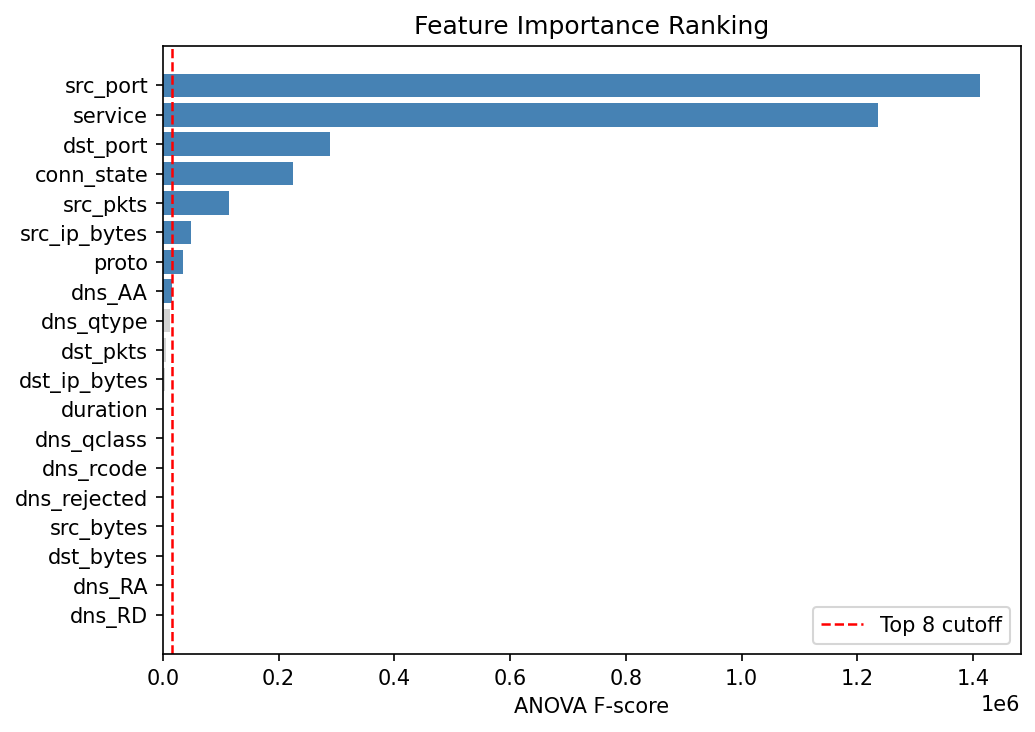
\includegraphics[width=0.75\textwidth]{figures/feature_importance.png}
    \caption{ANOVA F-score ranking of the 19 candidate features. The top~8 (blue) are selected for quantum encoding; the red dashed line marks the cutoff.}
    \label{fig:feature_importance}
\end{figure}

% ============================================================
\section{Handling Class Imbalance}
\label{sec:imbalance}

The severe class imbalance is problematic for training. Interpolation-based augmentation (e.g., SMOTE) is unsuitable here: a linear mix of two flows with different TCP flags or connection states produces a flow that cannot exist in practice. I instead use \emph{random undersampling} of the majority classes to match the minority (35,168~per class), giving a balanced dataset of 105,504~samples; quantum experiments subsample further due to simulation cost.

% ============================================================
\section{Normalization and Experimental Splits}
\label{sec:splits}

For angle encoding (Section~\ref{sec:qcnn}), each feature is scaled to $[0, \pi]$ via min-max normalization:
\begin{equation}
    x_i^{\text{scaled}} = \pi \cdot \frac{x_i - \min x_i}{\max x_i - \min x_i},
\end{equation}
so each feature spans the full range of a rotation gate. The scaler is fit on the training set only.

I define two experimental settings:

\textbf{Standard classification.} The balanced dataset is split 80/20 with stratified sampling (84,403 training / 21,101 test). All models share the same splits.

\textbf{Zero-day attack detection.} The model is trained on normal and DoS traffic only, then evaluated on injection attacks absent from training---simulating an unseen attack type (Figure~\ref{fig:zeroday_split}).

For quantum experiments, the standard 3-class split is stratified-subsampled to 500~training samples and 200~test samples, since circuit simulation on classical hardware scales linearly with dataset size. The zero-day quantum split uses fixed (non-stratified) random subsamples of the same size from the normal+DoS training set and the injection-only test set.

\begin{figure}[ht]
\centering
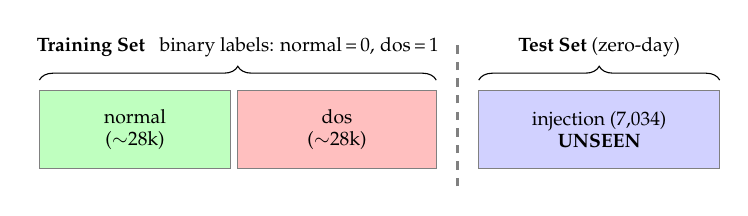
\begin{tikzpicture}[scale=0.9]
    % Training boxes
    \fill[green!25] (0,   0) rectangle (2.7, 1.1);
    \draw[gray]     (0,   0) rectangle (2.7, 1.1);
    \fill[red!25]   (2.8, 0) rectangle (5.6, 1.1);
    \draw[gray]     (2.8, 0) rectangle (5.6, 1.1);
    % Test box
    \fill[blue!18]  (6.2, 0) rectangle (9.6, 1.1);
    \draw[gray]     (6.2, 0) rectangle (9.6, 1.1);
    % Dashed separator
    \draw[dashed, thick, gray] (5.9, -0.25) -- (5.9, 1.85);
    % Labels inside boxes (two lines each)
    \node[align=center, font=\scriptsize] at (1.35, 0.55) {normal\\($\sim$28k)};
    \node[align=center, font=\scriptsize] at (4.2,  0.55) {dos\\($\sim$28k)};
    \node[align=center, font=\scriptsize] at (7.9,  0.55) {injection (7{,}034)\\\textbf{UNSEEN}};
    % Top braces
    \draw[decorate, decoration={brace,amplitude=5pt}] (0, 1.25) -- (5.6, 1.25)
        node[midway, above=5pt, font=\scriptsize]
        {\textbf{Training Set} \enspace binary labels: normal\,=\,0,\;dos\,=\,1};
    \draw[decorate, decoration={brace,amplitude=5pt}] (6.2, 1.25) -- (9.6, 1.25)
        node[midway, above=5pt, font=\scriptsize]
        {\textbf{Test Set} (zero-day)};
\end{tikzpicture}
\caption{Zero-day experimental split. The model trains on normal and DoS traffic only (binary classification), then is tested on injection attacks --- an entirely unseen class. High detection rate indicates genuine generalization beyond memorized attack patterns.}
\label{fig:zeroday_split}
\end{figure}

\chapter{Implementation}
\label{chap:implementation}

This chapter describes the implementation of all classifiers evaluated in this work. The full source code is publicly available~\cite{motamedifar2026repo} and organised in the \texttt{src/} directory, written in Python~3.11.

% ============================================================
\section{Software Environment}
\label{sec:env}

Three main libraries are used. \textbf{PennyLane}~\cite{pennylane} (v0.39) provides the QNode interface for circuit evaluation, the \texttt{lightning.qubit} noiseless simulator used in the main experiments, and the \texttt{AdamOptimizer}; gradients are computed with adjoint differentiation for speed. \textbf{scikit-learn}~\cite{sklearn} provides the classical classifiers and model-selection utilities. \textbf{pandas} and \textbf{NumPy} handle data loading and numerical operations. All experiments run on CPU under noiseless simulation; no real quantum hardware is used.

% ============================================================
\section{Classical Baselines}
\label{sec:impl_classical}

The classical baselines are implemented in \texttt{src/classical/classical\_baselines.py} and evaluated under both experimental settings defined in Section~\ref{sec:splits}.

\subsection{Support Vector Machine}

The SVM uses an RBF kernel. Hyperparameters $C \in \{0.1,\,1,\,10,\,100\}$ and $\gamma \in \{\texttt{scale},\,\texttt{auto},\,0.01,\,0.1\}$ are selected by 5-fold cross-validation on the training set. The best configuration is $C = 100$, $\gamma = \texttt{scale}$, achieving a cross-validation accuracy of 97.8\%.

\subsection{Random Forest}

A Random Forest of 100 decision trees is trained with default scikit-learn settings. As an ensemble method, it provides a robust baseline for tabular data and additionally yields feature importance scores that complement the ANOVA-based selection in the preprocessing stage.

\subsection{Neural Networks}

Two fully connected networks with ReLU activations are trained using Adam ($\eta = 10^{-3}$, up to 200 epochs):
\begin{itemize}[nosep]
    \item \textbf{NN-Small} ($8 \to 12 \to 6 \to 3$, ${\sim}207$ parameters): a small network in the same order of magnitude as the quantum classifiers.
    \item \textbf{NN-Medium} ($8 \to 16 \to 8 \to 3$, ${\sim}307$ parameters): a slightly larger network to test whether additional classical capacity helps.
\end{itemize}

\subsection{Autoencoder (Unsupervised Anomaly Detector)}
\label{sec:impl_autoencoder}

Supervised classifiers learn the boundary between the classes they are shown during training, which is precisely why they fail on unseen attack types. As a fairer classical baseline for the zero-day setting I add a shallow \emph{autoencoder} trained on normal traffic only. The architecture is a symmetric $8 \to 6 \to 3 \to 6 \to 8$ MLP with $\tanh$ activations and Xavier initialization, optimized with Adam ($\eta = 2 \times 10^{-3}$, weight decay $10^{-5}$, cosine learning-rate schedule) over 100~epochs on the ${\sim}28{,}000$ normal training samples. At inference, an input is flagged as anomalous if its reconstruction MSE exceeds the 95\textsuperscript{th} percentile of the training reconstruction errors. The threshold is set to the 95\textsuperscript{th} percentile of the training-normal reconstruction errors; the held-out normal split is used only to estimate the resulting false-positive rate, which is approximately 5\%. This protocol turns ``zero-day detection'' into ``anything that does not look like normal traffic,'' and is the standard unsupervised approach to network intrusion detection.

Table~\ref{tab:model_params} gives an overview of all models and their parameter budgets.

\begin{table}[ht]
\centering
\begin{tabular}{llc}
    \toprule
    \textbf{Model} & \textbf{Type} & \textbf{Parameters} \\
    \midrule
    SVM (RBF, $C{=}100$)          & Classical & kernel-based \\
    Random Forest (100 trees)      & Classical & tree-based   \\
    NN-Small $(12,6)$              & Classical & $\sim$207    \\
    NN-Medium $(16,8)$             & Classical & $\sim$307    \\
    Autoencoder $(8\!-\!6\!-\!3\!-\!6\!-\!8)$ & Classical & $\sim$160    \\
    \midrule
    Data Re-uploading (1 qubit, 6 layers)  & Quantum & 108 \\
    Data Re-uploading (4 qubits, 3 layers) & Quantum & 216 \\
    QCNN (8 qubits, 3 stages)             & Quantum & 81  \\
    \bottomrule
\end{tabular}
\caption{Parameter counts for all evaluated models. Quantum counts are the total for the 3-class one-vs-all system ($3\times$ the per-classifier count).}
\label{tab:model_params}
\end{table}

% ============================================================
\section{Quantum Classifiers}
\label{sec:impl_quantum}

Both quantum classifiers are implemented in \texttt{src/quantum/} using PennyLane's \texttt{lightning.qubit} simulator with adjoint differentiation, which gives identical results to \texttt{default.qubit} but runs noticeably faster. They share the same one-vs-all strategy: for $K = 3$ classes, three independent binary circuits are trained, each targeting one class with labels $y_i \in \{-1, +1\}$. At inference, the class whose circuit returns the highest $\langle Z \rangle$ is predicted.

\subsection{QCNN}

The QCNN operates on 8~qubits with 3~conv-pool stages ($8 \to 4 \to 2 \to 1$), followed by an $R_z R_y R_z$ fully connected layer on the remaining qubit. The convolutional unitary is a 6-parameter two-qubit block inspired by the ansatz family of Hur et al.~\cite{hur2022quantum}:
\[
U(\boldsymbol{\theta}) = \big[R_y R_z\big]_{q_1} \;\text{CNOT}\; \big[R_y R_z\big]_{q_0} \big[R_y R_z\big]_{q_1},
\]
a lighter variant of Hur et al.'s 10-parameter $U_6$ (which uses $R_x/R_z$ rotations and CRX entanglement). Each pooling layer uses a CRZ--CRY pair (2~parameters) to conditionally transfer information before discarding one qubit, a simplification of the CRZ + controlled-$R_x$ pooling proposed in the original paper. The total per-classifier parameter count is $3 \times 6 + 3 \times 2 + 3 = 27$, and $81$~parameters for the full 3-class system.

Input data is encoded via angle encoding: each of the 8~features is mapped to an $R_y$ rotation on the corresponding qubit.

\subsection{Data Re-uploading}

Two variants are implemented:
\begin{itemize}[nosep]
    \item \textbf{Single-qubit}: 6~layers on 1~qubit, $6 \times 6 = 36$~parameters per classifier (108~total).
    \item \textbf{Multi-qubit}: 3~layers on 4~qubits with nearest-neighbor CZ entanglement, $6 \times 4 \times 3 = 72$~parameters per classifier (216~total).
\end{itemize}

In each layer, rotation angles are computed as $\theta_j^{(l)} + w_j^{(l)} x_{f(j,l)}$, where the feature index $f(j,l)$ cycles through the input features across layers. For the multi-qubit variant, the output is the average $\langle Z \rangle$ over all qubits, expressed as a single Hamiltonian measurement $\langle H \rangle$ with $H = \frac{1}{n}\sum_q Z_q$.

\subsection{Training Configuration}

All quantum classifiers are trained with the Adam optimizer (learning rate $\eta = 0.01$) for 100~epochs. Each one-vs-all binary classifier uses a \emph{separate} optimizer instance to avoid momentum interference between sub-models. Gradients are computed via adjoint differentiation, which is mathematically equivalent to the parameter-shift rule but considerably faster in simulation. Parameters are initialized uniformly in $[-0.1, 0.1]$ with a controlled random seed to ensure reproducibility and to mitigate barren plateaus~\cite{mcclean2018barren}. To account for the known sensitivity of quantum circuits to initialization, the main experiments are repeated with 10~different seeds and results are reported as mean~$\pm$~standard deviation (Section~\ref{sec:res_sensitivity}). For the standard 3-class task, training uses a stratified subsample of 500~samples and test evaluation uses 200~stratified samples; for zero-day evaluation, the same sizes are drawn as fixed (non-stratified) random subsamples of the normal+DoS train set and the injection-only test set. All circuits run on noiseless simulation.

% ============================================================
\section{Evaluation Protocol}
\label{sec:eval_protocol}

All models are evaluated under the two settings defined in Section~\ref{sec:splits}:
\begin{itemize}[nosep]
    \item \textbf{Standard}: 3-class accuracy and weighted F1-score on the 200-sample test set.
    \item \textbf{Zero-day}: binary detection rate on the injection-only test set (7,034~samples after the 80/20 split), where the model has only seen normal and DoS traffic during training. Quantum models are evaluated on a fixed 200-sample subsample of this set due to simulation cost.
\end{itemize}
Results are reported in Chapter~\ref{chap:results}.

\chapter{Results}
\label{chap:results}

This chapter begins with a validation experiment that confirms the correctness of my quantum implementation (Section~\ref{sec:res_validation}), then presents the main results for standard classification (Section~\ref{sec:res_standard}) and zero-day attack detection (Section~\ref{sec:res_zeroday}). Section~\ref{sec:res_sensitivity} analyzes parameter initialization sensitivity, Section~\ref{sec:res_training} discusses training dynamics and ablation studies, and Section~\ref{sec:res_discussion} summarizes the findings. All quantum results are averaged over 10~random seeds; the autoencoder is also evaluated on 10~seeds. A consolidated table of all results is provided in Appendix~\ref{app:full_results}.

% ============================================================
\section{Implementation Validation}
\label{sec:res_validation}

Before evaluating on the IoT dataset, I validate the data re-uploading implementation on two standard synthetic benchmarks from the literature. P\'erez-Salinas et al.~\cite{perez2020data} report 90--98\% accuracy on similar 2D classification tasks. I train a single-qubit re-uploading circuit (4~layers, 24~parameters) for 80~epochs on 300~training samples from \texttt{make\_circles} and \texttt{make\_moons} (scikit-learn). Table~\ref{tab:res_validation} reports the results.

\begin{table}[ht]
\centering
\begin{tabular}{lccccc}
    \toprule
    \textbf{Dataset} & \textbf{Params} & \textbf{Accuracy} & \textbf{F1} & \textbf{MCC} \\
    \midrule
    \texttt{make\_circles} & 24 & 0.990 & 0.990 & 0.980 \\
    \texttt{make\_moons}   & 24 & 1.000 & 1.000 & 1.000 \\
    \bottomrule
\end{tabular}
\caption{Validation results on synthetic 2D datasets. My implementation achieves 99--100\% accuracy, consistent with the 90--98\% range reported by P\'erez-Salinas et al.~\cite{perez2020data}, confirming that the quantum circuit and training pipeline are correctly implemented.}
\label{tab:res_validation}
\end{table}

% ============================================================
\section{Standard Classification}
\label{sec:res_standard}

Table~\ref{tab:res_standard} reports accuracy, weighted F1-score, and Matthews Correlation Coefficient (MCC) on the 200-sample test set for the standard 3-class setting. MCC is included as it provides a balanced measure even when class sizes differ slightly~\cite{chicco2020advantages}. Quantum results are reported as mean~$\pm$~standard deviation over 10~random seeds (see Section~\ref{sec:res_sensitivity}).

\begin{table}[ht]
\centering
\begin{tabular}{llccc}
    \toprule
    \textbf{Model} & \textbf{Type} & \textbf{Accuracy} & \textbf{F1} & \textbf{MCC} \\
    \midrule
    Random Forest          & Classical & 0.990 & 0.990 & 0.985 \\
    SVM (RBF)              & Classical & 0.970 & 0.970 & 0.955 \\
    NN-Medium (16,\,8)     & Classical & 0.960 & 0.960 & 0.940 \\
    NN-Small (12,\,6)      & Classical & 0.925 & 0.925 & 0.888 \\
    \midrule
    Re-uploading 1q        & Quantum   & 0.752 $\pm$ 0.039 & 0.720 $\pm$ 0.051 & 0.662 $\pm$ 0.045 \\
    Re-uploading 4q        & Quantum   & 0.692 $\pm$ 0.011 & 0.654 $\pm$ 0.010 & 0.586 $\pm$ 0.016 \\
    QCNN (8q)              & Quantum   & 0.679 $\pm$ 0.025 & 0.636 $\pm$ 0.021 & 0.559 $\pm$ 0.043 \\
    \bottomrule
\end{tabular}
\caption{Standard 3-class results (normal / DoS / injection). Classical models are trained on 500 quantum-subset samples and tested on 200 samples. Quantum results are mean $\pm$ std over 10 seeds.}
\label{tab:res_standard}
\end{table}

All classical models achieve high accuracy ($\geq 92.5\%$), indicating strong class separation in the selected features. The quantum models perform significantly worse: the best quantum result is the single-qubit re-uploading at 75.2\% accuracy (MCC 0.66). The QCNN achieves 67.9\% with an MCC of 0.56.

These classical results are consistent with prior evaluations of ML models on ToN\_IoT: Moustafa~\cite{moustafa2021toniot} reports that tree-based and kernel methods consistently achieve $>$95\% accuracy on this dataset, confirming that our preprocessing pipeline and baseline implementation are correct.

This gap between classical and quantum is consistent with prior work showing that quantum classifiers do not outperform classical methods on datasets that are already linearly or near-linearly separable in the original feature space~\cite{schuld2021effect, bowles2024better}. With 8~well-chosen features, a Random Forest achieves 99\% accuracy with only 500~training samples, leaving no room for quantum advantage on this task.

% ============================================================
\section{Zero-Day Attack Detection}
\label{sec:res_zeroday}

Table~\ref{tab:res_zeroday} reports results on the zero-day setting, where models are trained exclusively on normal and DoS traffic and then tested on injection attacks---a class entirely absent from training. Since the test set is homogeneous (all injection), I report accuracy as the primary metric (equivalent to recall for the attack class). Quantum and autoencoder results are mean~$\pm$~std over 10~seeds.

\begin{table}[ht]
\centering
\begin{tabular}{llcc}
    \toprule
    \textbf{Model} & \textbf{Type} & \textbf{Accuracy} & \textbf{F1} \\
    \midrule
    Autoencoder (anomaly detection)        & Classical & \textbf{0.705 $\pm$ 0.144} & \textbf{0.819 $\pm$ 0.100} \\
    QCNN (8q), excl.\ barren-plateau seeds & Quantum   & \textbf{0.686 $\pm$ 0.068} & \textbf{0.812 $\pm$ 0.051} \\
    QCNN (8q), all 10 seeds                & Quantum   & 0.490 $\pm$ 0.305          & 0.587 $\pm$ 0.349 \\
    Re-uploading 1q                        & Quantum   & 0.092 $\pm$ 0.036          & 0.167 $\pm$ 0.058 \\
    Re-uploading 4q                        & Quantum   & 0.075 $\pm$ 0.023          & 0.138 $\pm$ 0.039 \\
    \midrule
    NN-Small (12,\,6)      & Classical & 0.028 & 0.054 \\
    SVM (RBF)              & Classical & 0.024 & 0.046 \\
    NN-Medium (16,\,8)     & Classical & 0.017 & 0.034 \\
    Random Forest          & Classical & 0.003 & 0.007 \\
    \bottomrule
\end{tabular}
\caption{Zero-day detection results. Models are trained on normal + DoS only; the test set contains exclusively injection attacks (unseen during training). Supervised classical models are evaluated on the full zero-day test set (7,034 samples); the autoencoder uses the same 7,034 samples as test set and is trained on all ${\sim}28{,}000$ normal samples; quantum models use a 200-sample test subsample and 500 training samples due to simulation cost. Autoencoder and quantum results are mean $\pm$ std over 10 seeds. The ``excl.\ barren-plateau seeds'' row reports the mean over the 7 seeds for which the QCNN converges; the 3 collapsed seeds $\{2, 5, 6\}$ (zero-day detection $\leq 9\%$) are excluded. Per-seed values are given in Table~\ref{tab:res_seeds} (Section~\ref{sec:res_sensitivity}).}
\label{tab:res_zeroday}
\end{table}

The results separate the seven evaluated models into three regimes:

\textbf{Supervised classical models fail completely.} Every supervised classical baseline (Random Forest, SVM, NN-Small, NN-Medium) detects fewer than 3\% of injection attacks. This is the expected behaviour: a classifier trained to discriminate \emph{normal} from \emph{DoS} learns a boundary tuned to those two distributions, and an unseen attack class lying away from that boundary is silently absorbed into one of the known classes.

\textbf{Two approaches reach $\sim$70\%.} The autoencoder (70.5\% $\pm$ 14.4\%) and the QCNN excluding barren-plateau seeds (68.6\% $\pm$ 6.8\%) reach essentially the same mean detection rate, an order of magnitude above the supervised classical baselines---but they are not both unsupervised. The autoencoder is trained on normal traffic only and flags any input that does not reconstruct well (genuine unsupervised anomaly detection). The QCNN is trained \emph{supervised} on normal-vs-DoS labels and happens to transfer to injection on 7 out of 10 initializations, suggesting that its quantum feature map captures a broader notion of ``not normal'' rather than memorizing the DoS distribution. Both approaches share the underlying intuition of modelling normal traffic and treating anything anomalous as an attack, but reach it through fundamentally different training regimes.

\textbf{Re-uploading remains brittle on zero-day.} Both re-uploading variants stay at 7--9\% on injection (versus ${\sim}2$--$3$\% for supervised classical), indicating they generalize slightly beyond their training classes but fall well short of the QCNN and the autoencoder. Their flatter feature maps appear to fit the specific DoS distribution rather than learning a broader notion of ``normal'' versus ``attack''.

The QCNN's headline number depends critically on whether barren-plateau seeds are included: across all 10 seeds the mean is 49.0\% with a 30.5\% standard deviation, masking a bimodal behaviour with 7~successful runs (54--76\%) and 3~training collapses ($\leq 9\%$). Section~\ref{sec:res_sensitivity} returns to this point. The autoencoder is more stable across seeds in terms of failure rate (1/10 vs.\ 3/10), but its detection rate when training succeeds varies more (std 14.4\% vs.\ 6.8\% for the QCNN).

A methodological note. The autoencoder is trained on all ${\sim}28{,}000$ normal samples while the quantum classifiers are restricted to the 500-sample quantum subsample for simulation-cost reasons (Chapter~\ref{chap:dataset}). The two methods therefore see different amounts of data, and this asymmetry should temper any direct numerical comparison. It does not, however, change the qualitative ranking observed: supervised classical $\ll$ re-uploading $<$ \{autoencoder, QCNN\}.

% ============================================================
\section{Initialization Sensitivity Analysis}
\label{sec:res_sensitivity}

The large standard deviation observed in QCNN zero-day performance motivated a systematic analysis of parameter initialization sensitivity. Table~\ref{tab:res_seeds} shows the per-seed QCNN results on the zero-day task (500 training samples, 100 epochs, 10 seeds).

\begin{table}[ht]
\centering
\begin{tabular}{lcccc}
    \toprule
    \textbf{Seed} & \textbf{Std.\ Acc.} & \textbf{Std.\ F1} & \textbf{ZD Acc.} & \textbf{ZD F1} \\
    \midrule
    0 & 0.720 & 0.674 & 0.755 & 0.860 \\
    1 & 0.675 & 0.638 & 0.640 & 0.780 \\
    2 & 0.625 & 0.593 & \textit{0.010} & \textit{0.020} \\
    3 & 0.685 & 0.616 & 0.730 & 0.844 \\
    4 & 0.680 & 0.641 & 0.695 & 0.820 \\
    5 & 0.690 & 0.650 & \textit{0.000} & \textit{0.000} \\
    6 & 0.665 & 0.629 & \textit{0.090} & \textit{0.165} \\
    7 & 0.680 & 0.642 & 0.710 & 0.830 \\
    8 & 0.660 & 0.625 & 0.730 & 0.844 \\
    9 & 0.710 & 0.651 & 0.540 & 0.701 \\
    \midrule
    Mean $\pm$ std (all 10)         & 0.679 $\pm$ 0.025 & 0.636 $\pm$ 0.021 & 0.490 $\pm$ 0.305 & 0.587 $\pm$ 0.349 \\
    Mean (excl.\ barren: 2,5,6) & 0.687 $\pm$ 0.019 & 0.641 $\pm$ 0.017 & 0.686 $\pm$ 0.068 & 0.812 $\pm$ 0.051 \\
    \bottomrule
\end{tabular}
\caption{Per-seed QCNN results (500 training samples, 100 epochs, 10 seeds). Standard accuracy is stable across seeds (66--72\%), but zero-day performance is bimodal: 7 seeds achieve 54--76\%, while 3 seeds (italics) collapse to $\leq 9\%$. The collapses are consistent with the barren plateau phenomenon~\cite{mcclean2018barren}.}
\label{tab:res_seeds}
\end{table}

Two observations emerge. \textbf{Standard classification is stable} across seeds (coefficient of variation 3.7\%); \textbf{zero-day detection is bimodal}, with 7/10 seeds reaching 54--76\% and 3 collapsing to $\leq 9\%$. This is consistent with the barren plateau phenomenon~\cite{mcclean2018barren}: gradient magnitudes vanish exponentially with circuit width, leaving the optimizer stuck in a flat region. The 30\% failure rate is not negligible---a single-seed evaluation could have produced either a strong false claim of quantum advantage or of total failure. Multi-seed evaluation is therefore not optional for variational quantum models. The re-uploading classifiers, by contrast, have a smoother landscape (coefficient of variation ${\sim}30\%$ on zero-day, ${\sim}5\%$ on standard) but also fail to generalize to the unseen class. The autoencoder has its own failure mode (1/10 seeds: near-identity reconstruction, detectable from a DoS sanity check), but at a meaningfully lower rate (10\% vs.\ 30\%).

% ============================================================
\section{Training Dynamics and Ablation Studies}
\label{sec:res_training}

Figure~\ref{fig:loss_curves} shows the training loss (MSE) over 100~epochs for the quantum models on the standard setting (seed~0).

\begin{figure}[ht]
\centering
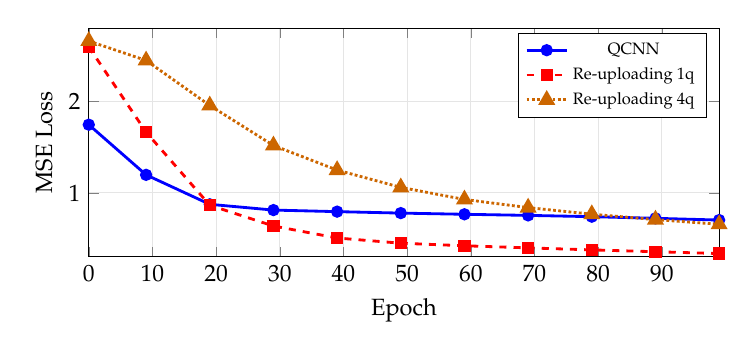
\begin{tikzpicture}[scale=0.85]
    \begin{axis}[
        xlabel={Epoch},
        ylabel={MSE Loss},
        xmin=0, xmax=99,
        ymin=0.3, ymax=2.8,
        legend style={at={(0.98,0.98)}, anchor=north east, font=\scriptsize},
        grid=major,
        grid style={gray!20},
        width=11cm, height=5cm,
    ]
    % QCNN standard (seed 0) -- solid + circle markers
    \addplot[blue, very thick, mark=*, mark size=2pt, mark options={solid, fill=blue}] coordinates {
        (0,1.745) (9,1.197) (19,0.875) (29,0.812) (39,0.795)
        (49,0.779) (59,0.766) (69,0.754) (79,0.740) (89,0.722) (99,0.703)
    };
    \addlegendentry{QCNN}

    % Re-uploading 1q standard (seed 0) -- dashed + square markers
    \addplot[red, very thick, dashed, mark=square*, mark size=2pt, mark options={solid, fill=red}] coordinates {
        (0,2.595) (9,1.664) (19,0.865) (29,0.638) (39,0.507)
        (49,0.450) (59,0.422) (69,0.399) (79,0.377) (89,0.357) (99,0.337)
    };
    \addlegendentry{Re-uploading 1q}

    % Re-uploading 4q standard (seed 0) -- dotted + triangle markers (darker orange for B&W readability)
    \addplot[orange!80!black, very thick, densely dotted, mark=triangle*, mark size=3pt, mark options={solid, fill=orange!80!black}] coordinates {
        (0,2.659) (9,2.447) (19,1.955) (29,1.518) (39,1.249)
        (49,1.060) (59,0.928) (69,0.839) (79,0.767) (89,0.708) (99,0.657)
    };
    \addlegendentry{Re-uploading 4q}
    \end{axis}
\end{tikzpicture}
\caption{Training loss curves for quantum models on the standard 3-class setting (100~epochs, 500~training samples, seed~0). All three models converge, with the single-qubit re-uploading reaching the lowest loss (0.34).}
\label{fig:loss_curves}
\end{figure}

All three quantum models show monotonically decreasing loss. The single-qubit re-uploading converges fastest, reaching a loss of 0.34 by epoch~99. The QCNN plateaus around epoch~30 and then decreases slowly to 0.70. The 4-qubit re-uploading model starts slowest but continues to improve throughout, reaching 0.66 by epoch~99.

The slower convergence of the 4-qubit model has three causes. First, its 72~parameters per classifier define a higher-dimensional loss landscape with more local minima. Second, the CZ entanglement gates create inter-qubit correlations that make individual parameter gradients less informative. Third, the averaged measurement $\langle H \rangle = \frac{1}{4}\sum_q Z_q$ dilutes the gradient signal compared to a single-qubit $\langle Z \rangle$. These effects are consistent with the barren plateau phenomenon~\cite{mcclean2018barren}.

\subsection{Ablation: Effect of Dataset Size}
\label{sec:res_ablation_data}

I investigate whether the quantum models benefit from additional training data by varying the number of training samples from 100 to 1000 (all with 100~epochs, seed~42). For datasets larger than 500~samples, I use mini-batch training (batch size 100). Table~\ref{tab:res_ablation_data} reports the resulting 3-class accuracy for each size.

\begin{table}[ht]
\centering
\begin{tabular}{lcccc}
    \toprule
    \textbf{Model} & $n=100$ & $n=250$ & $n=500$ & $n=1000$ \\
    \midrule
    Re-uploading 1q & 0.750 & 0.730 & 0.730 & 0.730 \\
    Re-uploading 4q & 0.695 & 0.700 & 0.680 & 0.700 \\
    QCNN (8q)       & 0.705 & 0.695 & 0.680 & 0.680 \\
    \midrule
    SVM (RBF)       & \multicolumn{4}{c}{0.970} \\
    Random Forest   & \multicolumn{4}{c}{0.990} \\
    \bottomrule
\end{tabular}
\caption{Standard 3-class accuracy vs.\ training set size (100~epochs, seed~42). All quantum models remain in the 68--75\% range regardless of dataset size, confirming that circuit capacity---not data---is the bottleneck.}
\label{tab:res_ablation_data}
\end{table}

All three quantum models are remarkably stable across dataset sizes (68--75\%), indicating that circuit capacity saturates with as few as 100~samples. No quantum model approaches the classical baselines. These results confirm that \emph{circuit capacity}, not training data, is the primary bottleneck for quantum classifiers on this task.

% ============================================================
\section{Discussion}
\label{sec:res_discussion}

The experiments yield three complementary findings: (i) classical baselines dominate on the standard task (99\% vs.\ 68--75\% for quantum, regardless of training budget), consistent with the expectation that quantum advantage is unlikely on classically separable data~\cite{schuld2021effect, bowles2024better}; (ii) on zero-day, supervised classical and supervised re-uploading both fail ($<3\%$ and 7--9\%), while two approaches---the unsupervised autoencoder (70.5\% $\pm$ 14.4\%, trained on normal traffic only) and the supervised QCNN excl.\ barren seeds (68.6\% $\pm$ 6.8\%, trained on normal-vs-DoS but transferring to injection)---succeed at comparable levels through very different mechanisms (reconstruction error vs.\ quantum feature separation); and (iii) the QCNN has lower variance when it trains (6.8\% vs.\ 14.4\%) but collapses 3/10 seeds vs.\ 1/10 for the autoencoder, and the 56$\times$ training-set asymmetry favours the autoencoder further. The QCNN's hierarchical pooling ($8 \to 1$) is what differentiates it from the re-uploading variants: same angle encoding, but multi-scale compression. The QCNN does not strictly dominate the autoencoder, but reaches comparable performance with 56$\times$ less training data---consistent with literature on quantum feature spaces and out-of-distribution generalization~\cite{havlicek2019supervised, schuld2020circuit}. Remaining limitations and perspectives are discussed in Chapter~\ref{chap:conclusion}.


% ============================================================
% Conclusion
% ============================================================
\OldSection{Conclusion}
\label{sec:conclusion}\label{chap:conclusion}

\OldSubsection*{Summary}

This work compared quantum machine learning classifiers with classical methods for IoT network intrusion detection, focusing on zero-day attacks. I evaluated five classical models (SVM, Random Forest, two neural networks, and an autoencoder anomaly detector) and three quantum architectures (QCNN, single- and 4-qubit data re-uploading) on ToN\_IoT, using a one-vs-all strategy over three classes (normal, DoS, injection). All quantum and autoencoder results are averaged over 10~seeds.

On the standard 3-class task, classical supervised models reached near-perfect accuracy (99\%) while quantum models plateaued at 68--75\% regardless of training budget. An ablation confirmed that \emph{circuit capacity}---not data---is the bottleneck: accuracy is nearly identical between 100 and 1000 training samples.

On the zero-day task, the picture inverted. Every supervised classical model failed ($<$~3\%), as did both re-uploading variants (7--9\%). Two approaches reached $\sim$70\%: the autoencoder at 70.5\% $\pm$ 14.4\% (trained unsupervised on normal traffic only), and the QCNN at 68.6\% $\pm$ 6.8\% on the 7 seeds that converged (49.0\% $\pm$ 30.5\% across all 10, with 3 barren-plateau collapses). The QCNN is trained \emph{supervised} on normal-vs-DoS labels but transfers to injection, suggesting its feature map captures a broader notion of ``not normal'' rather than memorizing the DoS class. The QCNN does not strictly dominate, but reaches comparable accuracy with 56$\times$ less training data and lower variance when convergent, at the cost of a 30\% training-failure rate (vs.\ 10\% for the autoencoder).

\OldSubsection*{Limitations}

All quantum experiments use a noiseless simulator (\texttt{lightning.qubit}), so real NISQ noise and decoherence are absent. QCNN zero-day accuracy varied from 0\% to 76\% across the 10 seeds, with 3 barren-plateau collapses---a single-seed run would have been misleading. The quantum models train on 500 samples and test on 200, while the autoencoder uses all ${\sim}28{,}000$ normal samples and the full 7,034 injection test set; this 56$\times$ asymmetry favours the autoencoder, so the two means are not a strict head-to-head. Finally, training used Adam with adjoint differentiation (mathematically equivalent to parameter-shift), without the advanced techniques (warm restarts, layer-wise pre-training, smart initialization) proposed in the literature to mitigate barren plateaus.

\OldSubsection*{Perspectives}

Several directions extend this work:

\begin{itemize}[nosep]
    \item \textbf{More seeds.} 30--50 seeds would tighten the confidence interval on the failure rate and enable significance testing against the autoencoder.
    \item \textbf{Barren-plateau mitigation.} Layer-wise pre-training, identity-block init, or warm-start strategies could reduce the 30\% failure rate---the single largest practical obstacle.
    \item \textbf{Noise simulation.} Realistic noise models (depolarizing, readout) would test whether the zero-day advantage survives under hardware conditions.
    \item \textbf{Larger circuits.} More qubits and depth could raise the capacity ceiling observed on the standard task.
    \item \textbf{Alternative encodings.} Amplitude or kernel-based encodings~\cite{havlicek2019supervised} would test whether the generalization is specific to angle encoding.
    \item \textbf{Real quantum hardware.} Execution on IBM Quantum or IonQ would ground-truth the simulator results.
    \item \textbf{Broader attack diversity.} Extending zero-day to backdoor, ransomware, or scanning attacks would test the generality of the anomaly-detection capability.
\end{itemize}

Despite classical methods' clear dominance on standard classification, the zero-day result offers an encouraging signal: both the QCNN and a classical autoencoder detect ${\sim}70\%$ of unseen attacks where every supervised classical model fails below 3\%. The QCNN does so with 56$\times$ less training data and lower variance when convergent, but pays a 30\% barren-plateau failure rate the autoencoder does not. The honest take-away is not ``quantum wins,'' but that quantum hierarchical feature maps and classical reconstruction-based detectors are two complementary routes to the same kind of out-of-distribution generalization---and the quantum route is not (yet) clearly preferable. If barren plateaus can be mitigated and the effect confirmed on noisy hardware and broader attack taxonomies, the quantum approach may become attractive where labelled normal traffic is scarce.

% ============================================================
% Acknowledgments
% ============================================================
\OldSection*{Acknowledgments}

I thank Fabrice Th\'{e}oleyre (ICube, CNRS / Universit\'{e} de Strasbourg) for supervising this research project and for detailed feedback on framing, methodology, and reporting. Code and reproduction scripts are available at
\url{https://github.com/ashkan-motamedifar/quantum-ml-ter}.

Parts of the text were refined with the assistance of a large language model for language formulation and proofreading. All scientific content---problem formulation, dataset preprocessing, model design, experiments, analyses, figures, and conclusions---is my own.

% ============================================================
% Appendix
% ============================================================
\appendix

\chapter{Complete Experimental Results}
\label{app:full_results}

Table~\ref{tab:features} lists the 19 features retained from the ToN\_IoT dataset after removing constant and identifier columns.

\begin{table}[ht]
    \centering
    \small
    \begin{tabular}{llp{7.5cm}}
        \toprule
        \textbf{Feature} & \textbf{Type} & \textbf{Description} \\
        \midrule
        src\_port, dst\_port  & Numerical & Source and destination transport port numbers \\
        proto                & Binary    & Transport protocol (TCP\,=\,0, UDP\,=\,1) \\
        service              & Categorical & Application service (none, DNS, HTTP, SSL) \\
        duration             & Numerical & Flow duration in seconds \\
        src\_bytes, dst\_bytes & Numerical & Bytes sent by source / destination \\
        conn\_state           & Categorical & TCP connection state (REJ, S0, SF, etc.) \\
        src\_pkts, dst\_pkts   & Numerical & Packets sent by source / destination \\
        src\_ip\_bytes, dst\_ip\_bytes & Numerical & IP-level bytes (including headers) \\
        dns\_qclass, dns\_qtype, dns\_rcode & Numerical & DNS query class, type, and response code \\
        dns\_AA, dns\_RD, dns\_RA, dns\_rejected & Binary & DNS flags (authoritative, recursion, etc.) \\
        \bottomrule
    \end{tabular}
    \caption{The 19 features retained after removing constant and identifier columns.}
    \label{tab:features}
\end{table}

Table~\ref{tab:full_results} consolidates all experimental results across models, tasks, and dataset sizes --- including the autoencoder for completeness. Classical supervised models use the full balanced training set. The autoencoder uses the full ${\sim}28{,}000$ normal samples and is averaged over 10~seeds. Quantum results at $n=500$ are mean~$\pm$~std over 10~seeds; other quantum sizes use seed~42 only.

\begin{table}[ht]
\centering
\small
\begin{tabular}{llcccc}
    \toprule
    \textbf{Model} & \textbf{Task} & $n=100$ & $n=250$ & $n=500$ & $n=1000$ \\
    \midrule
    \multicolumn{6}{l}{\textit{Classical supervised --- full training set (accuracy)}} \\
    \midrule
    Random Forest   & Standard  & \multicolumn{4}{c}{0.990} \\
    SVM (RBF)       & Standard  & \multicolumn{4}{c}{0.970} \\
    NN-Medium       & Standard  & \multicolumn{4}{c}{0.960} \\
    NN-Small        & Standard  & \multicolumn{4}{c}{0.925} \\
    \midrule
    NN-Small        & Zero-day  & \multicolumn{4}{c}{0.028} \\
    SVM (RBF)       & Zero-day  & \multicolumn{4}{c}{0.024} \\
    NN-Medium       & Zero-day  & \multicolumn{4}{c}{0.017} \\
    Random Forest   & Zero-day  & \multicolumn{4}{c}{0.003} \\
    \midrule
    \multicolumn{6}{l}{\textit{Classical unsupervised --- Autoencoder, ${\sim}28{,}000$ normal samples, 10 seeds (detection rate)}} \\
    \midrule
    Autoencoder     & Zero-day  & \multicolumn{4}{c}{\textbf{0.705 $\pm$ 0.144}} \\
    \midrule
    \multicolumn{6}{l}{\textit{Quantum --- Standard task, training subsamples of size $n$ (accuracy)}} \\
    \midrule
    Re-uploading 1q & Standard  & 0.750 & 0.730 & 0.752 $\pm$ 0.039 & 0.730 \\
    Re-uploading 4q & Standard  & 0.695 & 0.700 & 0.692 $\pm$ 0.011 & 0.700 \\
    QCNN (8q)       & Standard  & 0.705 & 0.695 & 0.679 $\pm$ 0.025 & 0.680 \\
    \midrule
    \multicolumn{6}{l}{\textit{Quantum --- Zero-day task, training subsamples of size $n$ (detection rate)}} \\
    \midrule
    QCNN (8q)       & Zero-day  & 0.005 & 0.020 & \textbf{0.490 $\pm$ 0.305} & 0.010 \\
    Re-uploading 1q & Zero-day  & 0.060 & 0.170 & 0.092 $\pm$ 0.036 & 0.105 \\
    Re-uploading 4q & Zero-day  & 0.040 & 0.040 & 0.075 $\pm$ 0.023 & 0.080 \\
    \bottomrule
\end{tabular}
\caption{Consolidated results across all models, tasks, and training-set sizes. \textbf{Classical supervised} models are trained on the full balanced training set and reported as single numbers. \textbf{The autoencoder} uses all ${\sim}28{,}000$ normal samples, is tested on the full 7,034-sample injection set, and is averaged over 10 seeds. \textbf{Quantum} models use subsamples of size $n$ (stratified for standard, fixed random for zero-day); $n=500$ results are mean $\pm$ std over 10 seeds, other sizes use seed~42 only. The QCNN zero-day values at $n\neq 500$ use seed~42, which lands in a barren plateau --- the multi-seed run at $n=500$ shows that 7/10 seeds actually achieve 54--76\% detection (mean 68.6\% $\pm$ 6.8\% excluding the 3 collapsed seeds).}
\label{tab:full_results}
\end{table}

The complete per-seed breakdown for the QCNN over 10~seeds is given in Table~\ref{tab:res_seeds} of Section~\ref{sec:res_sensitivity}. Re-uploading per-seed values are tightly clustered around their means (standard deviations of 0.039 and 0.011 on the standard task; 0.036 and 0.023 on zero-day) and are not reported individually.

% ---- Confusion Matrices ----

\section{Confusion Matrices}
\label{app:confusion}

Table~\ref{tab:cm_std_annex} shows confusion matrices for the best classical model (Random Forest) and the best quantum model (QCNN, seed~0) on the standard 3-class task. Table~\ref{tab:cm_zd_annex} shows the zero-day confusion matrices.

\begin{table}[ht]
\centering
\small
\begin{tabular}{c|ccc}
    \multicolumn{4}{c}{\textbf{Random Forest} --- Accuracy 0.990} \\
    \toprule
     & \textbf{pred.\ DoS} & \textbf{pred.\ Inj.} & \textbf{pred.\ Norm.} \\
    \midrule
    \textbf{DoS}    & 65 &  0 &  1 \\
    \textbf{Inj.}   &  0 & 67 &  0 \\
    \textbf{Norm.}   &  0 &  1 & 66 \\
    \bottomrule
\end{tabular}
\hspace{0.8cm}
\begin{tabular}{c|ccc}
    \multicolumn{4}{c}{\textbf{QCNN (seed 0)} --- Accuracy 0.720} \\
    \toprule
     & \textbf{pred.\ DoS} & \textbf{pred.\ Inj.} & \textbf{pred.\ Norm.} \\
    \midrule
    \textbf{DoS}    & 64 &  0 &  2 \\
    \textbf{Inj.}   &  0 & 64 &  3 \\
    \textbf{Norm.}   & 43 &  8 & 16 \\
    \bottomrule
\end{tabular}
\caption{Standard 3-class confusion matrices. The Random Forest achieves near-perfect separation. The QCNN correctly classifies DoS and injection but struggles with normal traffic, misclassifying 43 out of 67 normal samples as DoS.}
\label{tab:cm_std_annex}
\end{table}

\begin{table}[ht]
\centering
\small
\begin{tabular}{c|cc}
    \multicolumn{3}{c}{\textbf{QCNN (seed 0)} --- Zero-day Acc.\ 0.755} \\
    \toprule
     & \textbf{pred.\ Normal} & \textbf{pred.\ Attack} \\
    \midrule
    \textbf{Injection}  & 49 & 151 \\
    \bottomrule
\end{tabular}
\hspace{0.8cm}
\begin{tabular}{c|cc}
    \multicolumn{3}{c}{\textbf{Random Forest} --- Zero-day Acc.\ 0.003} \\
    \toprule
     & \textbf{pred.\ Normal} & \textbf{pred.\ Attack} \\
    \midrule
    \textbf{Injection}  & 7010 & 24 \\
    \bottomrule
\end{tabular}
\caption{Zero-day confusion matrices. The QCNN (seed~0) correctly detects 151 out of 200 unseen injection samples as attacks (75.5\%). The Random Forest detects only 24 out of 7,034 (0.3\%), classifying nearly all unseen attacks as normal.}
\label{tab:cm_zd_annex}
\end{table}

% ---- Seed Sensitivity Plot ----

\section{Initialization Sensitivity}
\label{app:sensitivity}

\begin{minipage}{\linewidth}
Figure~\ref{fig:seed_box} visualizes the effect of parameter initialization across 10~random seeds for each quantum model. The QCNN zero-day task shows extreme variance, with three seeds collapsing to near-random performance (barren plateau), while the standard task and re-uploading models remain stable.
\end{minipage}

\begin{figure}[ht]
\centering
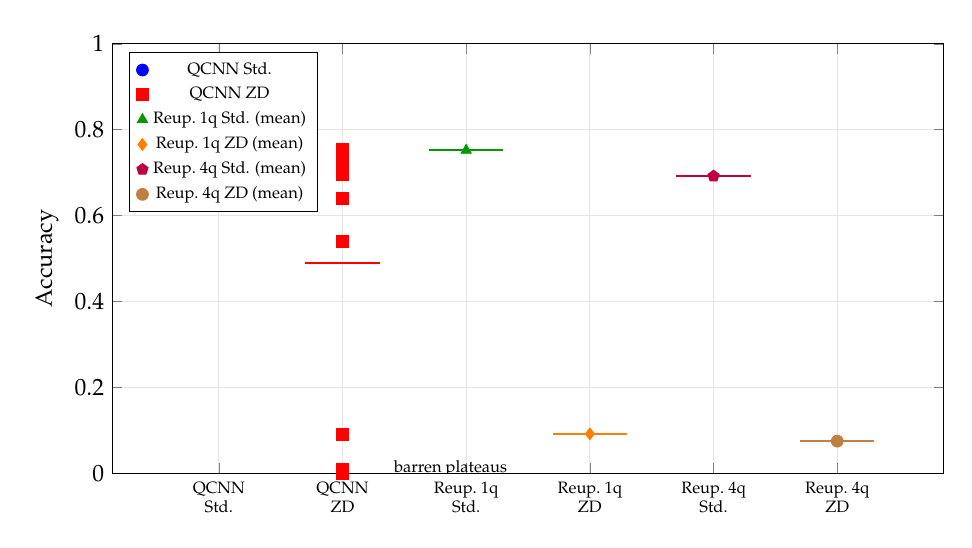
\begin{tikzpicture}[scale=0.85]
    \begin{axis}[
        ylabel={Accuracy},
        ymin=0, ymax=1.0,
        xtick={1,2,3,4,5,6},
        xticklabels={QCNN\\Std., QCNN\\ZD, Reup.~1q\\Std., Reup.~1q\\ZD, Reup.~4q\\Std., Reup.~4q\\ZD},
        x tick label style={align=center, font=\scriptsize},
        grid=major,
        grid style={gray!20},
        width=14cm, height=8cm,
        every axis plot/.append style={mark=*, mark size=2.5pt},
        legend style={at={(0.02,0.98)}, anchor=north west, font=\scriptsize},
    ]

    % QCNN Standard - 10 seeds
    \addplot[only marks, blue, mark=*] coordinates {
        (1, 0.720) (1, 0.675) (1, 0.625) (1, 0.685) (1, 0.680)
        (1, 0.690) (1, 0.665) (1, 0.680) (1, 0.660) (1, 0.710)
    };
    \addplot[blue, thick, no markers, forget plot] coordinates {(0.7, 0.679) (1.3, 0.679)};

    % QCNN Zero-day - 10 seeds
    \addplot[only marks, red, mark=square*] coordinates {
        (2, 0.755) (2, 0.640) (2, 0.010) (2, 0.730) (2, 0.695)
        (2, 0.000) (2, 0.090) (2, 0.710) (2, 0.730) (2, 0.540)
    };
    \addplot[red, thick, no markers, forget plot] coordinates {(1.7, 0.490) (2.3, 0.490)};

    % Reup 1q Standard - mean only (tightly clustered, std 0.039)
    \addplot[only marks, green!60!black, mark=triangle*] coordinates {(3, 0.752)};
    \addplot[green!60!black, thick, no markers, forget plot] coordinates {(2.7, 0.752) (3.3, 0.752)};

    % Reup 1q Zero-day
    \addplot[only marks, orange, mark=diamond*] coordinates {(4, 0.092)};
    \addplot[orange, thick, no markers, forget plot] coordinates {(3.7, 0.092) (4.3, 0.092)};

    % Reup 4q Standard
    \addplot[only marks, purple, mark=pentagon*] coordinates {(5, 0.692)};
    \addplot[purple, thick, no markers, forget plot] coordinates {(4.7, 0.692) (5.3, 0.692)};

    % Reup 4q Zero-day
    \addplot[only marks, brown, mark=otimes*] coordinates {(6, 0.075)};
    \addplot[brown, thick, no markers, forget plot] coordinates {(5.7, 0.075) (6.3, 0.075)};

    \node[black, font=\scriptsize, anchor=west] at (2.35, 0.010) {barren plateaus};

    \legend{QCNN Std., QCNN ZD, Reup.~1q Std. (mean), Reup.~1q ZD (mean), Reup.~4q Std. (mean), Reup.~4q ZD (mean)}
    \end{axis}
\end{tikzpicture}
\caption{Accuracy distribution across 10~random initialization seeds for each quantum model and task (500~samples, 100~epochs). QCNN points are individual seeds; re-uploading is shown as a single mean marker because its per-seed values are tightly clustered (standard deviations 0.011--0.039). The QCNN zero-day task exhibits three barren-plateau collapses at $\leq 9\%$, while seven seeds achieve 54--76\%. All other model--task combinations are stable across seeds.}
\label{fig:seed_box}
\end{figure}

% ---- Quantum Circuit Diagrams ----

\section{Quantum Circuit Architectures}
\label{app:circuits}

Figure~\ref{fig:qcnn_circuit} illustrates the QCNN architecture used in this work. The circuit operates on 8~qubits with 3~convolutional-pooling stages, progressively reducing the number of active qubits from 8 to 1.

\begin{figure}[ht]
\centering
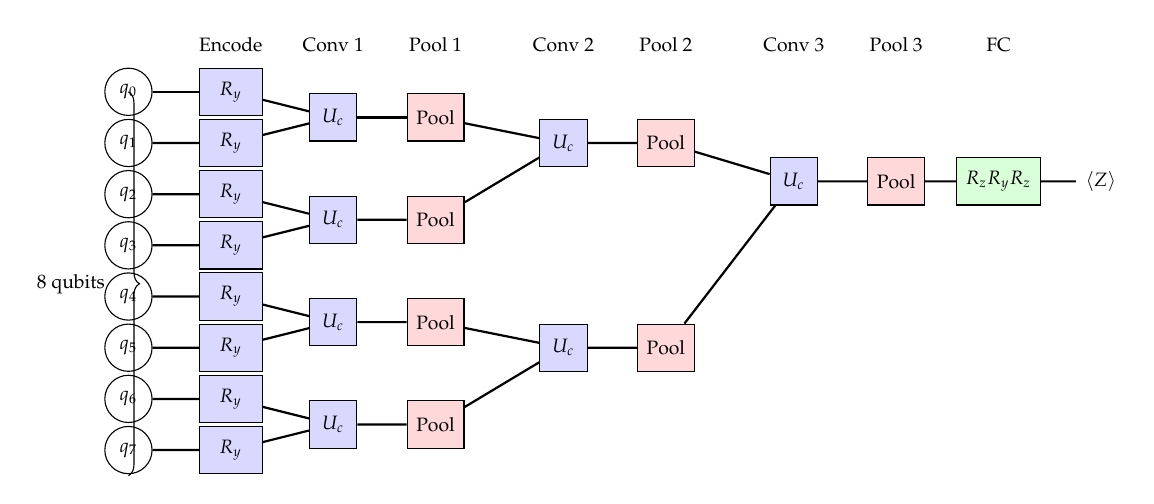
\begin{tikzpicture}[
    scale=0.65,
    qubit/.style={circle, draw, minimum size=6mm, inner sep=0pt, font=\scriptsize},
    gate/.style={rectangle, draw, fill=blue!15, minimum width=8mm, minimum height=6mm, font=\scriptsize},
    pool/.style={rectangle, draw, fill=red!15, minimum width=8mm, minimum height=6mm, font=\scriptsize},
    fc/.style={rectangle, draw, fill=green!15, minimum width=8mm, minimum height=6mm, font=\scriptsize},
    wire/.style={thick},
]
    % Qubits
    \foreach \i in {0,...,7} {
        \node[qubit] (q\i) at (0, -\i*1.0) {$q_{\i}$};
    }

    % Angle encoding
    \foreach \i in {0,...,7} {
        \node[gate] (enc\i) at (2, -\i*1.0) {$R_y$};
        \draw[wire] (q\i) -- (enc\i);
    }
    \node[font=\scriptsize, above] at (2, 0.6) {Encode};

    % Conv layer 1 (8 qubits)
    \foreach \i/\j in {0/1, 2/3, 4/5, 6/7} {
        \node[gate, minimum width=6mm] (c1\i) at (4, {-(\i+\j)/2*1.0}) {$U_c$};
        \draw[wire] (enc\i) -- (c1\i);
        \draw[wire] (enc\j) -- (c1\i);
    }
    \node[font=\scriptsize, above] at (4, 0.6) {Conv~1};

    % Pool layer 1 (8 -> 4)
    \foreach \i/\j in {0/1, 2/3, 4/5, 6/7} {
        \node[pool, minimum width=6mm] (p1\i) at (6, {-(\i+\j)/2*1.0}) {Pool};
        \draw[wire] (c1\i) -- (p1\i);
    }
    \node[font=\scriptsize, above] at (6, 0.6) {Pool~1};

    % Conv layer 2 (4 qubits)
    \foreach \i/\j in {0/2, 4/6} {
        \node[gate, minimum width=6mm] (c2\i) at (8.5, {-(\i+\j)/2*1.0}) {$U_c$};
        \draw[wire] (p1\i) -- (c2\i);
        \draw[wire] (p1\j) -- (c2\i);
    }
    \node[font=\scriptsize, above] at (8.5, 0.6) {Conv~2};

    % Pool layer 2 (4 -> 2)
    \foreach \i/\j in {0/2, 4/6} {
        \node[pool, minimum width=6mm] (p2\i) at (10.5, {-(\i+\j)/2*1.0}) {Pool};
        \draw[wire] (c2\i) -- (p2\i);
    }
    \node[font=\scriptsize, above] at (10.5, 0.6) {Pool~2};

    % Conv layer 3 (2 qubits)
    \node[gate, minimum width=6mm] (c3) at (13, -1.75) {$U_c$};
    \draw[wire] (p20) -- (c3);
    \draw[wire] (p24) -- (c3);
    \node[font=\scriptsize, above] at (13, 0.6) {Conv~3};

    % Pool layer 3 (2 -> 1)
    \node[pool, minimum width=6mm] (p3) at (15, -1.75) {Pool};
    \draw[wire] (c3) -- (p3);
    \node[font=\scriptsize, above] at (15, 0.6) {Pool~3};

    % FC layer
    \node[fc, minimum width=6mm] (fc) at (17, -1.75) {$R_z R_y R_z$};
    \draw[wire] (p3) -- (fc);
    \node[font=\scriptsize, above] at (17, 0.6) {FC};

    % Measurement
    \node[font=\scriptsize] (meas) at (19, -1.75) {$\langle Z \rangle$};
    \draw[wire] (fc) -- (meas);

    % Dimension labels
    \draw[decorate, decoration={brace, amplitude=4pt, mirror}] (0, -7.5) -- (0, 0.0)
        node[midway, left=5pt, font=\scriptsize] {8 qubits};
\end{tikzpicture}
\caption{QCNN architecture ($8 \to 4 \to 2 \to 1$ qubits). Input features are encoded via $R_y$ rotations. Three convolutional-pooling stages hierarchically reduce the circuit width. Each convolutional unitary $U_c$ applies 6~parameterized rotations; each pooling layer uses CRZ--CRY (2~parameters) to transfer information before discarding one qubit. A final $R_z R_y R_z$ layer on the remaining qubit produces the output $\langle Z \rangle \in [-1, +1]$. Total: 27~parameters per binary classifier.}
\label{fig:qcnn_circuit}
\end{figure}

Figure~\ref{fig:reup_circuit} illustrates the single-qubit data re-uploading circuit.

\begin{figure}[ht]
\centering
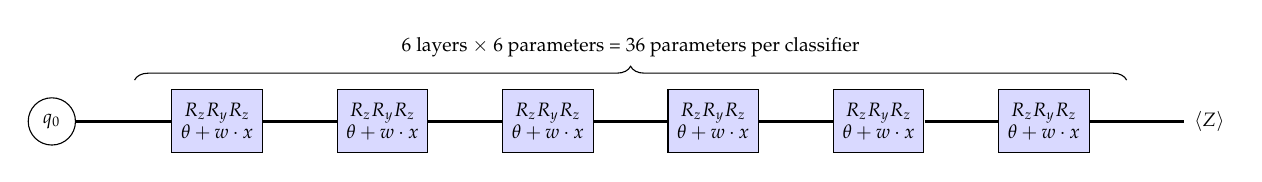
\begin{tikzpicture}[
    scale=0.75,
    qubit/.style={circle, draw, minimum size=6mm, inner sep=0pt, font=\scriptsize},
    gate/.style={rectangle, draw, fill=blue!15, minimum width=10mm, minimum height=8mm, font=\scriptsize, align=center},
    wire/.style={thick},
]
    % Single qubit
    \node[qubit] (q) at (0, 0) {$q_0$};

    % Layers
    \foreach \l [count=\i from 1] in {1,2,3,4,5,6} {
        \pgfmathsetmacro{\x}{\i * 2.8}
        \node[gate] (layer\l) at (\x, 0) {$R_z R_y R_z$\\$\theta + w \cdot x$};
        \ifnum\i=1
            \draw[wire] (q) -- (layer\l);
        \else
            \pgfmathtruncatemacro{\prev}{\l-1}
            \draw[wire] (layer\prev) -- (layer\l);
        \fi
    }

    % Measurement
    \node[font=\scriptsize] (meas) at (19.6, 0) {$\langle Z \rangle$};
    \draw[wire] (layer6) -- (meas);

    % Brace
    \draw[decorate, decoration={brace, amplitude=5pt}] (2.8-1.4, 0.7) -- (16.8+1.4, 0.7)
        node[midway, above=5pt, font=\scriptsize] {6 layers $\times$ 6 parameters = 36 parameters per classifier};

\end{tikzpicture}
\caption{Single-qubit data re-uploading circuit (6~layers). Each layer applies parameterized $R_z R_y R_z$ rotations where the rotation angles are $\theta_j^{(l)} + w_j^{(l)} \cdot x_{f(j,l)}$, combining trainable weights with input features that cycle across layers. The same qubit is reused across all layers, enabling a single qubit to learn complex decision boundaries. Total: 36~parameters per binary classifier.}
\label{fig:reup_circuit}
\end{figure}

Figure~\ref{fig:reup_multi_circuit} shows the multi-qubit variant used in this work: 4~qubits with 3~re-uploading layers and nearest-neighbor CZ entanglement between layers.

\begin{figure}[ht]
\centering
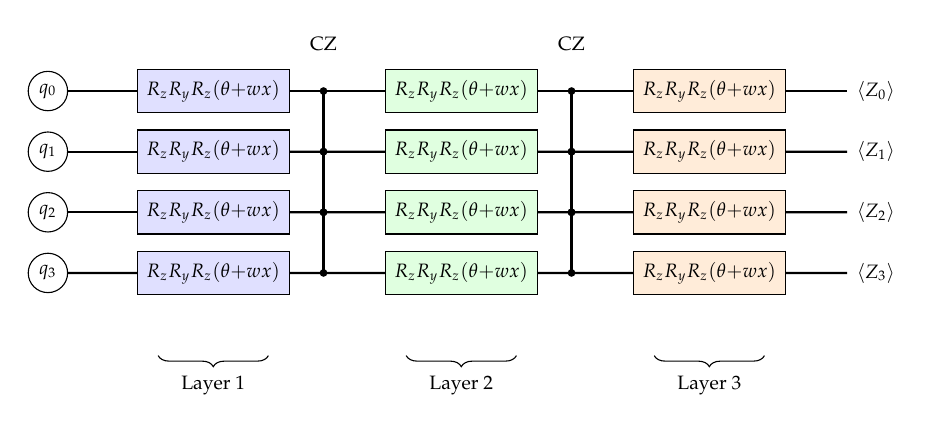
\begin{tikzpicture}[
    scale=0.7,
    qubit/.style={circle, draw, minimum size=5mm, inner sep=0pt, font=\scriptsize},
    gate/.style={rectangle, draw, fill=blue!12, minimum width=16mm, minimum height=5.5mm, font=\scriptsize, align=center},
    wire/.style={thick},
]
    % Qubit labels
    \foreach \q in {0,1,2,3} {
        \node[qubit] (q\q) at (0, -\q*1.1) {$q_\q$};
    }

    % Layer 1 gates
    \foreach \q in {0,1,2,3} {
        \node[gate] (l1q\q) at (3, -\q*1.1) {$R_z R_y R_z(\theta{+}wx)$};
        \draw[wire] (q\q) -- (l1q\q);
    }

    % CZ entanglement 1
    \foreach \q in {0,1,2} {
        \pgfmathtruncatemacro{\qq}{\q+1}
        \draw[thick] (5, -\q*1.1) -- (5, -\qq*1.1);
        \fill (5, -\q*1.1) circle (0.07);
        \fill (5, -\qq*1.1) circle (0.07);
    }
    \node[above, font=\scriptsize] at (5, 0.55) {CZ};
    \foreach \q in {0,1,2,3} {
        \draw[wire] (l1q\q) -- (5, -\q*1.1);
    }

    % Layer 2 gates
    \foreach \q in {0,1,2,3} {
        \node[gate, fill=green!12] (l2q\q) at (7.5, -\q*1.1) {$R_z R_y R_z(\theta{+}wx)$};
        \draw[wire] (5, -\q*1.1) -- (l2q\q);
    }

    % CZ entanglement 2
    \foreach \q in {0,1,2} {
        \pgfmathtruncatemacro{\qq}{\q+1}
        \draw[thick] (9.5, -\q*1.1) -- (9.5, -\qq*1.1);
        \fill (9.5, -\q*1.1) circle (0.07);
        \fill (9.5, -\qq*1.1) circle (0.07);
    }
    \node[above, font=\scriptsize] at (9.5, 0.55) {CZ};
    \foreach \q in {0,1,2,3} {
        \draw[wire] (l2q\q) -- (9.5, -\q*1.1);
    }

    % Layer 3 gates
    \foreach \q in {0,1,2,3} {
        \node[gate, fill=orange!15] (l3q\q) at (12, -\q*1.1) {$R_z R_y R_z(\theta{+}wx)$};
        \draw[wire] (9.5, -\q*1.1) -- (l3q\q);
    }

    % Final CZ + measurement
    \foreach \q in {0,1,2,3} {
        \draw[wire] (l3q\q) -- (14.5, -\q*1.1);
        \node[right, font=\scriptsize] at (14.5, -\q*1.1) {$\langle Z_{\q} \rangle$};
    }

    % Layer braces below
    \draw[decorate, decoration={brace, amplitude=4pt, mirror}] (2.0, -4.8) -- (4.0, -4.8)
        node[midway, below=4pt, font=\scriptsize] {Layer~1};
    \draw[decorate, decoration={brace, amplitude=4pt, mirror}] (6.5, -4.8) -- (8.5, -4.8)
        node[midway, below=4pt, font=\scriptsize] {Layer~2};
    \draw[decorate, decoration={brace, amplitude=4pt, mirror}] (11.0, -4.8) -- (13.0, -4.8)
        node[midway, below=4pt, font=\scriptsize] {Layer~3};
\end{tikzpicture}
\caption{Multi-qubit data re-uploading circuit (4~qubits, 3~layers). Each qubit independently applies parameterized $R_z R_y R_z$ rotations that mix input data $\mathbf{x}$ with trainable weights, with nearest-neighbor CZ gates entangling the qubits between layers. The final output is the average of the per-qubit $\langle Z \rangle$ measurements, expressed as a single Hamiltonian measurement $\langle H \rangle = \tfrac{1}{n}\sum_q Z_q$. Total: $6 \times 4 \times 3 = 72$~parameters per binary classifier.}
\label{fig:reup_multi_circuit}
\end{figure}


% ============================================================
% Bibliography
% ============================================================
\bibliographystyle{unsrtnat}
\bibliography{references}

\end{document}
